% ============================================================
%  Chapter 14 — Disciplined Convex Programming
%  Algorithms for Optimization, 2nd ed. (2026)
%  Kochenderfer & Wheeler
%  Reader-friendly edition: self-contained prose, Greek-letter
%  pronunciations, notation blocks, worked numerical examples.
% ============================================================
\documentclass[aspectratio=169,10pt]{beamer}

\usetheme{Madrid}
\usecolortheme{seahorse}

\usepackage{amsmath,amssymb,amsfonts}
\usepackage{mathtools}
\usepackage{graphicx}
\usepackage{booktabs}
\usepackage{listings}
\usepackage{xcolor}
\usepackage{tikz}
\usetikzlibrary{arrows.meta,positioning,shapes.geometric,fit}
\usepackage{array}
\usepackage{multicol}
\usepackage{colortbl}

\graphicspath{{figures/}}

% ── listings style ──────────────────────────────────────────
\lstset{
  language=Python,
  basicstyle=\ttfamily\scriptsize,
  numbers=left,
  numberstyle=\tiny\color{gray},
  frame=single,
  backgroundcolor=\color{gray!7},
  keywordstyle=\color{blue!70!black}\bfseries,
  commentstyle=\color{green!50!black}\itshape,
  stringstyle=\color{red!60!black},
  breaklines=true,
  showstringspaces=false,
  tabsize=4,
  captionpos=b,
}

% ── color definitions ────────────────────────────────────────
\definecolor{dcpblue}{RGB}{44,106,173}
\definecolor{dcpgreen}{RGB}{58,125,58}
\definecolor{dcporange}{RGB}{196,144,10}
\definecolor{dcpred}{RGB}{192,57,43}
\definecolor{lightgray}{RGB}{245,245,245}

% ── footline ────────────────────────────────────────────────
\setbeamertemplate{footline}[frame number]

% ── title ───────────────────────────────────────────────────
\title[Ch.14 Disciplined Convex Programming]{%
  Chapter 14\\[4pt]
  \textbf{Disciplined Convex Programming}}
\subtitle{\textit{Algorithms for Optimization}, 2nd ed.\ (2026)\\
  Kochenderfer \& Wheeler}
\author{Lecture Slides}
\date{}

% ============================================================
\begin{document}
% ============================================================

% ── Title slide ─────────────────────────────────────────────
\begin{frame}
  \titlepage
\end{frame}

% ── Outline ─────────────────────────────────────────────────
\begin{frame}{Chapter Outline}
  \tableofcontents
\end{frame}

% ============================================================
\section{Canonical Form of a DCP}
% ============================================================

\begin{frame}[allowframebreaks]{What is Disciplined Convex Programming?}

  Convex optimization problems have a special structure: a \textbf{convex
  objective function} and either convex inequality constraints or
  \emph{affine} (linear) equality constraints.  When these conditions hold,
  any local minimum is guaranteed to be a \emph{global} minimum, which is
  an extraordinarily powerful property.  However, before we can exploit
  this guarantee, we must first \emph{verify} that the problem is indeed
  convex --- and doing this by hand is surprisingly difficult for realistic
  problems.

  \begin{block}{The Core Challenge}
    Checking convexity of an expression by hand requires applying calculus
    rules (second derivative tests, composition theorems, etc.) to every
    sub-expression in the problem.  As problems grow in size this becomes
    tedious, error-prone, and impractical to automate in an ad-hoc fashion.
    We need a \emph{systematic} framework.
  \end{block}

  \begin{alertblock}{DCP: Disciplined Convex Programming --- Definition}
    A \textbf{disciplined convex program (DCP)} is a convex optimization
    problem written according to a set of grammatical rules such that
    \emph{automated software can verify its convexity} and then
    \emph{transcribe it into a standard canonical form} accepted by
    high-performance numerical solvers.  The word ``disciplined'' means
    the problem writer follows the grammar; the word ``programming'' here
    means mathematical programming (optimization), not computer
    programming.
  \end{alertblock}

  \begin{columns}
    \begin{column}{0.55\textwidth}
      The figure on the right illustrates the overall workflow: a user
      writes a problem using DCP syntax, the system checks the grammar
      (verification), converts it to canonical form (canonicalization),
      and passes it to a solver.  The key insight is that \emph{atoms}
      --- a library of primitive functions with known mathematical
      properties --- provide the building blocks for every expression.
    \end{column}
    \begin{column}{0.42\textwidth}
      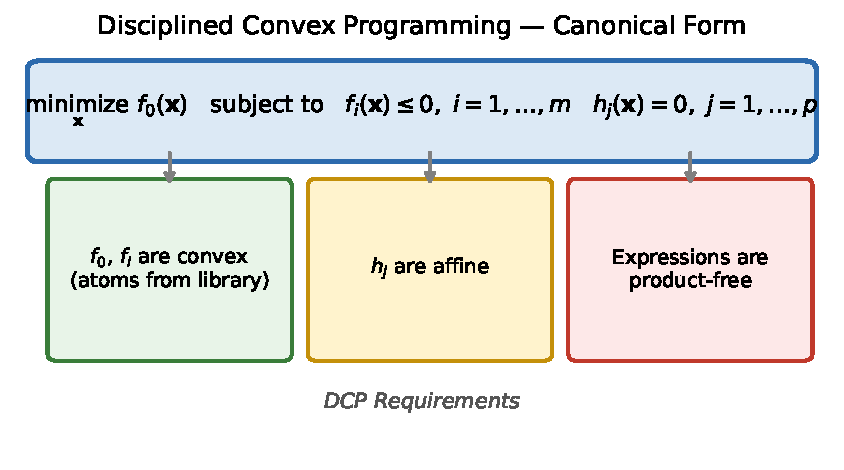
\includegraphics[width=\textwidth]{fig_dcp_canonical.pdf}
    \end{column}
  \end{columns}

  \begin{alertblock}{Key Insight}
    DCP separates the task of \emph{modelling} (writing the
    problem) from the task of \emph{solving} (running the numerical
    algorithm).  The user never needs to hand-derive gradients or
    reformulations; the DCP system handles all of that automatically.
  \end{alertblock}

\end{frame}

% ────────────────────────────────────────────────────────────
\begin{frame}[allowframebreaks]{Canonical Form of a DCP}

  Every convex optimization problem, no matter how it is originally
  stated, can be cast into a \emph{standard form} that unambiguously
  specifies the objective and constraints.  This standard form is what
  DCP targets.

  \begin{block}{Standard Convex Problem (Eq.\ 14.1)}
    \[
      \underset{\mathbf{x}}{\mathrm{minimize}}\quad f_0(\mathbf{x})
      \qquad
      \text{subject to}\quad
      \begin{cases}
        f_i(\mathbf{x}) \leq 0 & i = 1,\ldots,m\\
        h_j(\mathbf{x}) = 0    & j = 1,\ldots,p
      \end{cases}
    \]
  \end{block}

  \begin{block}{Notation}
    \begin{itemize}
      \item $\mathbf{x} \in \mathbb{R}^n$ (``x bold in R\,n'') is the
            \emph{decision variable} --- an $n$-dimensional vector of real
            numbers that we are choosing to minimise the objective.
      \item $f_0(\mathbf{x})$ is the \emph{objective function}: the
            quantity we want to make as small as possible.  DCP requires
            $f_0$ to be \textbf{convex}.
      \item $f_i(\mathbf{x})$ (``f sub i of x'') are the
            \emph{inequality constraint functions} for $i = 1, \ldots, m$
            (i.e., the first through the $m$-th constraint).  Each $f_i$
            must also be \textbf{convex}, so the feasible region
            $\{f_i(\mathbf{x}) \leq 0\}$ is a convex set.
      \item $h_j(\mathbf{x})$ (``h sub j of x'') are the
            \emph{equality constraint functions} for $j = 1, \ldots, p$.
            These must be \textbf{affine} (i.e., of the form
            $\mathbf{a}^\top \mathbf{x} - b$) because an equality
            constraint is simultaneously an upper and lower bound, which
            forces the function to be both convex and concave --- only
            affine functions have both properties.
      \item $m$ is the number of inequality constraints; $p$ is the
            number of equality constraints; $n$ is the number of
            decision variables.
    \end{itemize}
  \end{block}

  \begin{alertblock}{How to Read This Formula}
    We are searching over all possible vectors $\mathbf{x}$ in
    $n$-dimensional space for the one that makes $f_0(\mathbf{x})$
    smallest, while staying in the feasible region defined by the
    constraints.  Because all constraint sets are convex, the feasible
    region is itself convex, and because $f_0$ is convex over a convex
    domain, there is exactly one globally optimal solution (or a convex
    set of equally optimal solutions).
  \end{alertblock}

  \begin{block}{The Four DCP Requirements}
    A problem must satisfy four conditions before DCP tools will accept
    it:
    \begin{enumerate}
      \item \textbf{Product-free expressions.}  No expression in the
            problem may contain the \emph{product} of two non-constant
            sub-expressions.  For example, $x_1 \cdot x_2$ is forbidden
            because neither factor is a fixed number.  This restriction
            guarantees that curvature can be tracked symbolically.
      \item \textbf{Top-level production rules.}  The top-level role of
            each expression must match its curvature: the objective of a
            minimisation must be convex; the left-hand side of an
            inequality $\leq 0$ must be convex; equality constraint
            functions must be affine.
      \item \textbf{Sign rules.}  The system tracks whether each constant
            coefficient is positive or negative, because multiplying a
            convex function by $-1$ makes it concave (and vice versa).
      \item \textbf{Composition rules.}  When one function is applied to
            the output of another (function composition), the DCP system
            checks whether the curvature and monotonicity of the outer
            function are compatible with the curvature of the inner
            expression.
    \end{enumerate}
  \end{block}

\end{frame}

% ────────────────────────────────────────────────────────────
\begin{frame}[allowframebreaks]{Running Example (Ex.\ 14.1)}

  To make the abstract definitions concrete, let us trace through a
  specific problem and verify step-by-step that it is a valid DCP.

  \begin{exampleblock}{The Problem}
    \[
      \underset{\mathbf{x}}{\mathrm{minimize}}\;
      \|\mathbf{A}\mathbf{x} - \mathbf{b}\|_1
      \qquad
      \text{subject to}\;
      \|\mathbf{C}\mathbf{x} - \mathbf{d}\|_{1.5} \leq 3
    \]
    with specific numerical matrices:
    \[
      \mathbf{A}=\begin{bmatrix}2&-1\\1&3\end{bmatrix},\quad
      \mathbf{b}=\begin{bmatrix}4\\-5\end{bmatrix},\quad
      \mathbf{C}=\begin{bmatrix}0&1\\3&-4\end{bmatrix},\quad
      \mathbf{d}=\begin{bmatrix}-1\\0\end{bmatrix}
    \]
  \end{exampleblock}

  \begin{block}{Notation for This Example}
    \begin{itemize}
      \item $\mathbf{x} \in \mathbb{R}^2$ is the two-dimensional decision
            vector we are optimising.
      \item $\mathbf{A}$ and $\mathbf{C}$ are $2 \times 2$ matrices of
            fixed coefficients (given numbers, not variables).
      \item $\mathbf{b}$ and $\mathbf{d}$ are fixed two-dimensional
            vectors.
      \item $\|\cdot\|_1$ (``L1 norm'' or ``one-norm'') of a vector
            $\mathbf{v}$ equals $|v_1| + |v_2| + \cdots + |v_n|$, i.e.,
            the sum of the absolute values of all components.
      \item $\|\cdot\|_{1.5}$ is the $L_p$ norm with $p = 1.5$, defined
            as $\bigl(\sum_i |v_i|^{1.5}\bigr)^{1/1.5}$.  Any $L_p$
            norm with $p \geq 1$ is convex.
      \item The constraint $\|\mathbf{C}\mathbf{x} - \mathbf{d}\|_{1.5}
            \leq 3$ says: ``the $L_{1.5}$ distance between
            $\mathbf{C}\mathbf{x}$ and $\mathbf{d}$ must be at most 3.''
    \end{itemize}
  \end{block}

  \begin{block}{Step-by-step DCP Verification}
    \begin{itemize}
      \item The expression $\mathbf{A}\mathbf{x} - \mathbf{b}$ is
            \textbf{affine} (a matrix--vector product of a fixed matrix
            $\mathbf{A}$ with the variable $\mathbf{x}$, minus a
            constant vector).  Affine expressions are both convex and
            concave.
      \item Applying the $L_1$ norm $\|\cdot\|_1$ to an affine argument
            gives a \textbf{convex} function.  This follows from the atom
            library: norms are convex, and composing a convex function
            that is nondecreasing in absolute value with an affine
            argument preserves convexity.
      \item Similarly, $\mathbf{C}\mathbf{x} - \mathbf{d}$ is affine,
            and applying $\|\cdot\|_{1.5}$ gives a convex function.
      \item The constraint \emph{convex function} $\leq$ \emph{constant}
            satisfies the DCP rule for inequality constraints.
      \item The objective is \emph{minimise convex function}, which is
            exactly what DCP requires.
    \end{itemize}
    \textcolor{dcpgreen}{\textbf{Conclusion: this is a valid DCP.}}
  \end{block}

  \begin{alertblock}{Key Insight}
    The power of DCP is that each check above can be performed
    \emph{mechanically} by software, consulting only the atom library
    for curvature information.  The human writer never needs to invoke
    the definition of convexity directly.
  \end{alertblock}

\end{frame}

% ────────────────────────────────────────────────────────────
\begin{frame}[allowframebreaks]{The Atom Library}

  The entire DCP framework rests on a library of \emph{atoms}: primitive
  mathematical functions whose curvature, monotonicity, domain, and range
  have been catalogued in advance.  When you write a DCP expression, you
  are composing atoms according to grammar rules, just as you compose
  words according to language rules.

  \begin{columns}
    \begin{column}{0.55\textwidth}
      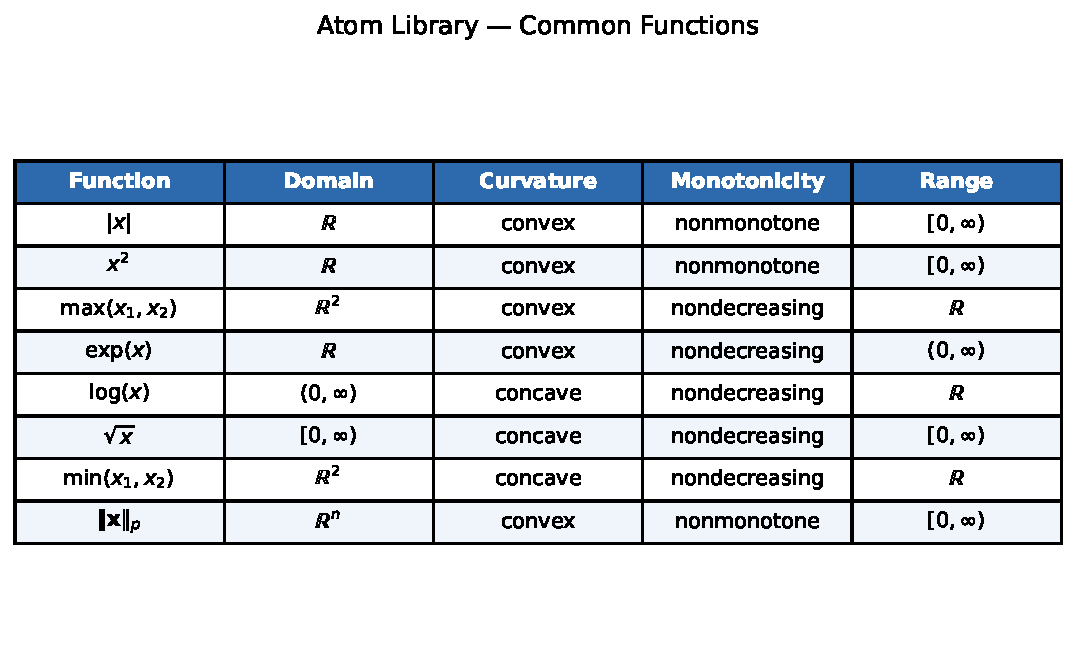
\includegraphics[width=\textwidth]{fig_atom_library.pdf}
    \end{column}
    \begin{column}{0.42\textwidth}
      \begin{block}{What Every Atom Provides}
        For each atom $f$ in the library, the following information is
        stored:
        \begin{itemize}
          \item \textbf{Domain} --- the set of input values for which $f$
                is defined.  For example, $\log(x)$ has domain
                $x > 0$.
          \item \textbf{Curvature} --- whether $f$ is convex, concave,
                or affine (linear).
          \item \textbf{Monotonicity} (per argument) --- whether $f$ is
                nondecreasing or nonincreasing in each of its arguments
                over its effective domain.  This is essential for the
                composition rule.
          \item \textbf{Range} --- bounds on the possible output values
                of $f$.  For example, $\sqrt{x} \geq 0$ always.
        \end{itemize}
      \end{block}
    \end{column}
  \end{columns}

  \medskip

  \begin{block}{Examples of Common Atoms and Their Properties}
    \small
    \begin{tabular}{lllll}
      \toprule
      \textbf{Atom} & \textbf{Notation} & \textbf{Curvature} &
        \textbf{Monotonicity} & \textbf{Domain}\\
      \midrule
      Absolute value  & $|x|$            & Convex   & Nonincreasing ($x\!<\!0$), nondecreasing ($x\!>\!0$) & $\mathbb{R}$\\
      Square          & $x^2$            & Convex   & Same as $|x|$ & $\mathbb{R}$\\
      Square root     & $\sqrt{x}$       & Concave  & Nondecreasing & $x\geq 0$\\
      Logarithm       & $\log(x)$        & Concave  & Nondecreasing & $x > 0$\\
      Exponential     & $e^x$            & Convex   & Nondecreasing & $\mathbb{R}$\\
      $L_p$ norm      & $\|\mathbf{v}\|_p$ & Convex & ---  & $\mathbb{R}^n$, $p\!\geq\!1$\\
      Maximum         & $\max(a,b)$      & Convex   & Nondecreasing & $\mathbb{R}$\\
      \bottomrule
    \end{tabular}
  \end{block}

  \begin{block}{Sets as Atoms}
    Sets can also be treated as atoms.  For example:
    \begin{itemize}
      \item The real line $\mathbb{R}^n$ is trivially a convex set.
      \item The positive orthant $\mathbb{R}^n_+ = \{\mathbf{x} : x_i \geq 0\}$
            (``R-n-plus'') is a convex set, used to represent
            non-negativity constraints.
      \item The \emph{epigraph} (``epi'') and \emph{hypograph} (``hypo'')
            of a function (defined later) are convex sets associated
            with convex and concave functions respectively.
    \end{itemize}
  \end{block}

\end{frame}

% ============================================================
\section{Verification of Convexity}
% ============================================================

\begin{frame}[allowframebreaks]{Verification --- The Two-Stage Pipeline}

  Given a problem written in DCP notation, the software must determine
  whether it actually satisfies the convexity requirements.  This
  verification is done in two sequential stages.

  \begin{block}{Two-Stage Verification}
    \begin{enumerate}
      \item \textbf{Stage 1 --- Product-free check.}  The system scans
            every expression in the problem and confirms that no
            expression contains the product of two non-constant
            sub-expressions.  This stage is purely syntactic: it does
            not reason about curvature at all, only about the structure
            of the formula.
      \item \textbf{Stage 2 --- Rule checking.}  The system walks the
            \emph{expression tree} (the tree-shaped representation of
            the formula) from the leaves up to the root, assigning a
            curvature label (convex / concave / affine / neither) to
            each node, and verifying the sign, composition, and
            top-level production rules at each step.
    \end{enumerate}
  \end{block}

  \begin{columns}
    \begin{column}{0.48\textwidth}
      Both stages are fully automatic.  If either stage fails, the
      system reports an error with a pointer to the offending
      sub-expression, allowing the user to fix the formulation.
      If both stages pass, the problem is a valid DCP and can proceed to
      canonicalization.
    \end{column}
    \begin{column}{0.48\textwidth}
      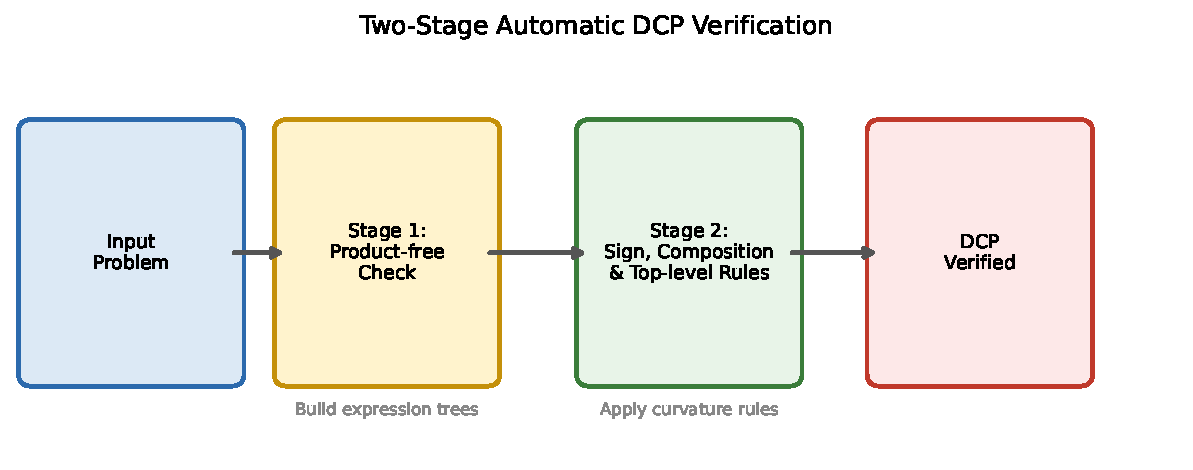
\includegraphics[width=\textwidth]{fig_verification_pipeline.pdf}
    \end{column}
  \end{columns}

\end{frame}

% ────────────────────────────────────────────────────────────
\begin{frame}[allowframebreaks]{Product-Free Expressions}

  The product-free requirement is the first filter in DCP verification.
  Its purpose is to ensure that every expression can be written as a
  \emph{linear combination} of atom outputs, which makes curvature
  analysis tractable.

  \begin{block}{Definition: Product-Free Expression (Eq.\ 14.5)}
    An expression $e$ is called \textbf{product-free} if and only if it
    can be written in the form:
    \[
      e \;=\; a \;+\; \mathbf{b}^\top\mathbf{x}
              \;+\; \sum_{j=1}^{q} c_j \, f_j(\mathbf{e}_j)
    \]
  \end{block}

  \begin{block}{Notation}
    \begin{itemize}
      \item $a \in \mathbb{R}$ is a real-valued constant (a fixed
            number).
      \item $\mathbf{b} \in \mathbb{R}^n$ (``b bold in R-n'') is a
            constant vector of coefficients.
      \item $\mathbf{b}^\top\mathbf{x}$ (``b-transpose times x'') denotes
            the inner product $b_1 x_1 + b_2 x_2 + \cdots + b_n x_n$,
            which is an affine (linear) function of $\mathbf{x}$.
      \item $\sum_{j=1}^{q}$ (``sigma from j equals 1 to q'', meaning
            ``sum over'') denotes the sum of $q$ terms, one for each
            atom call.
      \item $c_j$ is a \emph{constant} scalar coefficient for the
            $j$-th atom call (it can be positive, negative, or zero,
            but it must not involve any variable).
      \item $f_j$ is the $j$-th atom from the atom library (e.g.,
            $\log$, $\|\cdot\|_2$, $\max$).
      \item $\mathbf{e}_j$ (``e bold sub j'') is the vector of
            \emph{sub-expressions} passed as arguments to $f_j$.
            Crucially, each component of $\mathbf{e}_j$ must itself be
            a product-free expression (the definition is recursive).
    \end{itemize}
  \end{block}

  \begin{alertblock}{How to Read This Definition}
    This says: a product-free expression is a constant, plus a
    linear term in the variables, plus a weighted sum of atom
    evaluations.  The only operations allowed are addition,
    subtraction, and scalar multiplication by constants --- no
    variable-times-variable products.  This is what makes symbolic
    curvature tracking possible.
  \end{alertblock}

  \begin{columns}
    \begin{column}{0.48\textwidth}
      \begin{exampleblock}{Product-Free (Valid DCP) Examples}
        \begin{itemize}
          \item $3 + 2x_1 + \log(x_2)$: constant $3$, linear
                term $2x_1$, atom $\log(x_2)$ --- product-free.
          \item $\max(x_1^2 - 3,\; x_2)$: the $\max$ atom with
                sub-expressions $x_1^2 - 3$ (using the \texttt{square}
                atom for $x_1^2$) and $x_2$ --- product-free.
          \item $\|\mathbf{A}\mathbf{x} - \mathbf{b}\|_2$: the $L_2$
                norm atom applied to an affine expression --- product-free.
        \end{itemize}
      \end{exampleblock}
    \end{column}
    \begin{column}{0.48\textwidth}
      \begin{alertblock}{Not Product-Free (Invalid DCP) Examples}
        \begin{itemize}
          \item $x_1 \cdot x_2$: product of two variables --- not
                allowed.
          \item $x_1^2$ written as $x_1 \times x_1$: same problem.
                However, $x_1^2$ \emph{is} allowed if written as
                \texttt{square}$(x_1)$, i.e., using the designated
                atom.
          \item $\sin(x_1) \cdot \log(x_2)$: product of two
                non-constant sub-expressions --- not allowed.
        \end{itemize}
      \end{alertblock}
    \end{column}
  \end{columns}

  \begin{block}{Important Note on $x^2$}
    The expression $x^2$ seems like a product, but DCP handles it
    through the \texttt{square} atom, which stores the curvature
    information (convex, nondecreasing for $x \geq 0$, nonincreasing
    for $x \leq 0$) directly.  The atom library is the bridge that
    allows nonlinear functions while still maintaining the product-free
    property.
  \end{block}

\end{frame}

% ────────────────────────────────────────────────────────────
\begin{frame}[allowframebreaks]{Sign Rules for Curvature}

  Once an expression passes the product-free check, the system assigns
  curvature labels by applying sign rules.  These rules govern how
  scalar multiplication and addition affect the convexity or concavity
  of expressions.

  \begin{block}{Sign Rules for Scaling}
    Let $f(\mathbf{x})$ be a function with known curvature, and let $c$
    be a \emph{constant} scalar.  Then:
    \begin{itemize}
      \item If $f$ is \textbf{convex} and $c > 0$ (positive), then
            $c \cdot f(\mathbf{x})$ is \textbf{convex}.  Scaling a bowl
            shape upward keeps it a bowl.
      \item If $f$ is \textbf{convex} and $c < 0$ (negative), then
            $c \cdot f(\mathbf{x})$ is \textbf{concave}.  Flipping a
            bowl upside down gives an arch.
      \item If $f$ is \textbf{concave} and $c > 0$, then
            $c \cdot f(\mathbf{x})$ is \textbf{concave}.
      \item If $f$ is \textbf{concave} and $c < 0$, then
            $c \cdot f(\mathbf{x})$ is \textbf{convex}.
    \end{itemize}
  \end{block}

  \begin{block}{Sum Rules}
    Adding two functions affects curvature as follows:
    \begin{columns}
      \begin{column}{0.48\textwidth}
        \begin{itemize}
          \item convex $+$ convex $=$ \textbf{convex}
          \item concave $+$ concave $=$ \textbf{concave}
          \item affine $+$ convex $=$ \textbf{convex}
          \item affine $+$ concave $=$ \textbf{concave}
        \end{itemize}
      \end{column}
      \begin{column}{0.48\textwidth}
        \begin{itemize}
          \item convex $+$ concave $=$ \textbf{neither} (in general)
          \item affine $+$ affine $=$ \textbf{affine}
        \end{itemize}
      \end{column}
    \end{columns}
    The intuition: mixing a bowl and an arch in the same sum does not
    guarantee any curvature.
  \end{block}

  \begin{exampleblock}{Worked Example: Classifying $3 + 2\log(1+x_1) - \sin(x_2)$}
    Assume $x_1 \geq 0$ so that $1 + x_1 \geq 1 > 0$ (keeping $\log$
    in its domain), and $x_2 \in [-\pi, 0]$.

    \textbf{Step 1.}  $\log(1+x_1)$ is a concave function (the natural
    logarithm is always concave on its domain).

    \textbf{Step 2.}  Multiplying by the positive constant $2$: the
    term $2\log(1+x_1)$ is \textbf{concave} (positive constant times
    concave is concave).

    \textbf{Step 3.}  The sine function $\sin(x_2)$ on
    $x_2 \in [-\pi, 0]$ has a non-positive second derivative
    throughout, so $\sin(x_2)$ is \textbf{convex} on this interval.

    \textbf{Step 4.}  The term $-\sin(x_2)$ multiplies a convex
    function by $-1$ (a negative constant), making it
    \textbf{concave}.

    \textbf{Step 5.}  Adding: $3$ (affine) $+$ $2\log(1+x_1)$
    (concave) $+$ $(-\sin(x_2))$ (concave) is the sum of an affine
    and two concave terms, which is \textbf{concave}.

    \textbf{Conclusion:} the whole expression is \textbf{concave}
    on the specified domain.
  \end{exampleblock}

\end{frame}

% ────────────────────────────────────────────────────────────
\begin{frame}[allowframebreaks]{Composition Rules}

  The composition rule handles the most common pattern in practice:
  applying one function to the output of another.  For example,
  $1/g(\mathbf{x})$ composes the reciprocal function $f(t) = 1/t$ with
  $g(\mathbf{x})$.  The composition rule tells us when $f(g(\mathbf{x}))$
  is convex or concave based on the properties of $f$ and $g$.

  \begin{block}{Composition Theorem for Convexity (Eqs.\ 14.3--14.4)}
    The composed function $f(\varepsilon_1, \ldots, \varepsilon_m)$ (where
    $\varepsilon$ (epsilon) denotes each sub-expression argument) is
    \textbf{convex} if:
    \begin{itemize}
      \item $f$ is either affine or convex; \emph{and}
      \item For each argument $\varepsilon_i$ (``epsilon sub i'',
            meaning the $i$-th argument):
        \begin{itemize}
          \item[$\triangleright$] $f$ is \emph{nondecreasing} in
                $\varepsilon_i$ over its effective range $\mathcal{R}$
                (``R, the range''), \emph{and} $\varepsilon_i$ is
                itself \textbf{convex}; \textbf{or}
          \item[$\triangleright$] $f$ is \emph{nonincreasing} in
                $\varepsilon_i$ over $\mathcal{R}$, \emph{and}
                $\varepsilon_i$ is itself \textbf{concave}; \textbf{or}
          \item[$\triangleright$] $\varepsilon_i$ is \textbf{affine}
                (no monotonicity condition needed for affine arguments).
        \end{itemize}
    \end{itemize}
    Mirror rules apply symmetrically for establishing \textbf{concavity}
    of $f$.
  \end{block}

  \begin{alertblock}{How to Read This Theorem}
    Think of it in terms of direction: a convex outer function
    ``pointing up'' combined with a convex inner function also
    ``pointing up'' via a nondecreasing connection stays convex.
    A convex outer function ``pointing up'' combined with a concave
    inner function ``pointing down'' through a nonincreasing (sign-
    flipping) connection also preserves convexity, because two
    ``flips'' cancel.
  \end{alertblock}

  \begin{block}{Decomposition Consequence (Eq.\ 14.7)}
    When $f$ is convex and nondecreasing, the constraint
    $f(g(\mathbf{x})) \leq y$ can be split into two simpler
    constraints:
    \[
      f(g(\mathbf{x})) \leq y \quad\iff\quad
      \begin{cases}f(z) \leq y\\[4pt]g(\mathbf{x}) \leq z\end{cases}
    \]
    where $z$ (``z'') is a fresh auxiliary variable.  This
    decomposition is valid because $f$ is nondecreasing: if
    $g(\mathbf{x}) \leq z$ and $f(z) \leq y$, then
    $f(g(\mathbf{x})) \leq f(z) \leq y$.  This splitting technique
    is the basis of canonicalization (Section~3).
  \end{block}

\end{frame}

% ────────────────────────────────────────────────────────────
\begin{frame}[allowframebreaks]{Composition Rule --- Worked Examples}

  Two worked examples trace the composition theorem to its conclusion.

  \begin{columns}
    \begin{column}{0.50\textwidth}
      \begin{exampleblock}{Ex.\ 14.3: Is $f(g(\mathbf{x})) = 1/g(\mathbf{x})$ convex?}
        Here $f(t) = 1/t$ (the reciprocal function) and
        $g(\mathbf{x}) = 3 + 2\log(1+x_1) - \sin(x_2)$.

        \textbf{Step 1.}  From the previous example, $g$ is
        \textbf{concave} with range $\subseteq [3, \infty)$:
        \begin{align*}
          \mathrm{range}(g)
          &\;\subseteq\; 3 + 2\cdot\mathrm{range}(\log(1+x_1)) - \sin(x_2)\\
          &\;=\; [3,3] + [0,\infty) + [0,1] \;=\; [3,\infty)
        \end{align*}

        \textbf{Step 2.}  $f(t) = 1/t$ is \textbf{convex and
        nonincreasing} for $t > 0$.

        \textbf{Step 3.}  Apply composition rule: $f$ is convex
        and \emph{nonincreasing}, and $g$ is \emph{concave} --- this
        matches the second sub-case (nonincreasing outer, concave
        inner).

        \textbf{Step 4.}  Also verify the range: $f$ is
        nonincreasing on $(0, \infty)$, and the range of $g$ is
        $[3,\infty) \subset (0,\infty)$, so the range condition
        holds.

        \textcolor{dcpgreen}{\textbf{Conclusion:}} $1/g(\mathbf{x})$
        is \textbf{convex}.
      \end{exampleblock}
    \end{column}
    \begin{column}{0.47\textwidth}
      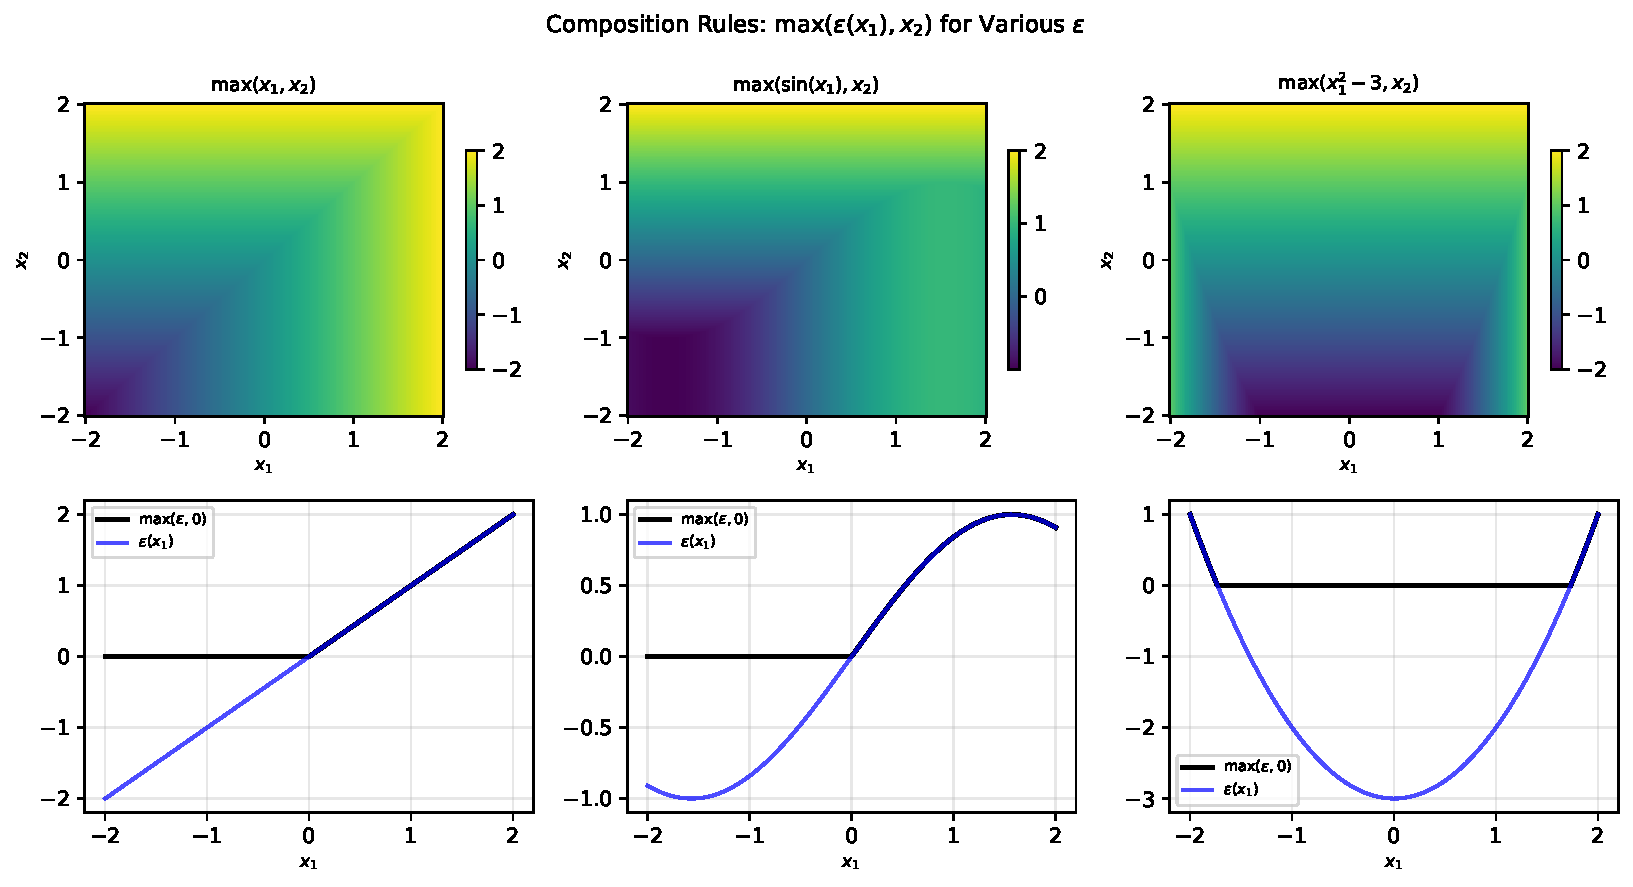
\includegraphics[width=\textwidth]{fig_composition_max.pdf}
      \vspace{-4pt}
      \begin{block}{Ex.\ 14.5: Is $\max(\varepsilon(x_1), x_2)$ convex?}
        \small
        The $\max$ function is convex and nondecreasing in both
        arguments.  For the first argument $\varepsilon$:
        \begin{itemize}
          \item $\varepsilon = x_1$ (affine): $\max(x_1, x_2)$ is
                \textbf{convex}.
          \item $\varepsilon = \sin(x_1)$ (neither convex nor
                concave in general): composition rule fails ---
                \textbf{not convex}.
          \item $\varepsilon = x_1^2 - 3$ (convex via
                \texttt{square} atom): $\max$ is nondecreasing,
                argument is convex --- \textbf{convex}.
          \item $\varepsilon = \log(x_1) - 1$ (concave, since
                $\log$ is concave): $\max$ is nondecreasing but
                argument is concave --- rule fails ---
                \textbf{not convex}.
        \end{itemize}
      \end{block}
    \end{column}
  \end{columns}

\end{frame}

% ────────────────────────────────────────────────────────────
\begin{frame}[allowframebreaks]{Top-Level Production Rules}

  After assigning curvature labels to all sub-expressions, the DCP
  system checks the \emph{top-level} role of each expression: is it
  an objective to be minimised, an objective to be maximised, an
  inequality constraint left-hand side, or an equality constraint?
  Each role has a curvature requirement.

  \begin{block}{Top-Level Curvature Requirements}
    \begin{tabular}{lll}
      \toprule
      \textbf{Context} & \textbf{Required curvature} & \textbf{Example}\\
      \midrule
      Minimise $f_0$ & $f_0$ must be \textbf{convex}
        & $\min\;\|\mathbf{x}\|_2$\\
      Maximise $f_0$ & $f_0$ must be \textbf{concave}
        & $\max\;\log(\det X)$\\
      Inequality $f_i(\mathbf{x}) \leq c$ & $f_i$ must be \textbf{convex},
        $c$ must be \textbf{concave}
        & $g(\mathbf{x})\leq 0$\\
      Inequality $c \leq f_i(\mathbf{x})$ & $c$ must be \textbf{convex},
        $f_i$ must be \textbf{concave}
        & $0\leq h(\mathbf{x})$\\
      Equality $h_j(\mathbf{x}) = 0$ & $h_j$ must be \textbf{affine}
        & $\mathbf{A}\mathbf{x}=\mathbf{b}$\\
      \bottomrule
    \end{tabular}
  \end{block}

  \begin{alertblock}{Why Must Equality Constraints Be Affine?}
    An equality constraint $f(\mathbf{x}) = 0$ is equivalent to two
    simultaneous inequality constraints: $f(\mathbf{x}) \leq 0$ AND
    $f(\mathbf{x}) \geq 0$.  The first requires $f$ to be
    \emph{convex}; the second requires $f$ to be \emph{concave}.  The
    only functions that are simultaneously convex and concave are the
    \textbf{affine} functions.  This is why DCP forbids nonlinear
    equality constraints.
  \end{alertblock}

  \begin{exampleblock}{Example: What happens with a nonlinear equality?}
    Suppose someone writes $x_1^2 + x_2^2 = 1$ (the unit circle) as
    an equality constraint.  The function $f(\mathbf{x}) = x_1^2 +
    x_2^2$ is convex but \emph{not} concave, so it cannot satisfy both
    inequality requirements simultaneously.  The DCP system will reject
    this constraint.  The correct way to handle such constraints is to
    use them as \emph{inequalities} (e.g., $x_1^2 + x_2^2 \leq 1$) or
    to reformulate the problem entirely.
  \end{exampleblock}

\end{frame}

% ────────────────────────────────────────────────────────────
\begin{frame}[allowframebreaks]{Automatic Verification --- Expression Tree (Ex.\ 14.6)}

  The expression tree is the internal data structure that DCP software
  uses to represent a formula.  Each leaf is a variable or constant;
  each internal node is an operation or atom; the root represents the
  whole expression.  Verification is a single bottom-up pass of the
  tree, assigning curvature labels as it goes.

  \begin{columns}
    \begin{column}{0.52\textwidth}
      \begin{exampleblock}{Problem}
        \small
        \[
          \underset{x_1,x_2}{\mathrm{minimize}}\;
          \mathrm{pow}(a_1x_1+a_2x_2-b_1,\,2)
        \]
        \[
          \text{s.t.}\quad c_1x_1+c_2x_2=d,\quad
          \sqrt{\min(x_1,x_2)}\geq 1-\log(x_2)
        \]
        where $a_1, a_2, b_1, c_1, c_2, d$ are known constants.
      \end{exampleblock}
      \begin{block}{Verification Tree (Simplified Trace)}
        \small
        \texttt{minimize}\\
        \quad$\hookrightarrow$ \texttt{pow}($\varepsilon$,\,2):
          \textcolor{dcpblue}{convex} (squaring is convex)\\
        \quad\quad$\hookrightarrow$ $-b_1+a_1x_1+a_2x_2$:
          \textcolor{dcpblue}{affine} (linear in $x_1, x_2$)\\
        \texttt{subject to}\\
        \quad$\hookrightarrow$ \texttt{=}: affine = affine \checkmark\\
        \quad$\hookrightarrow$ \texttt{$\geq$}: concave $\geq$ convex \checkmark\\
        \quad\quad$\hookrightarrow$ $\sqrt{\varepsilon}$:
          \textcolor{dcpgreen}{concave, nondecreasing}\\
        \quad\quad\quad$\hookrightarrow$ $\min(\varepsilon,\varepsilon)$:
          \textcolor{dcpgreen}{concave, nondecreasing}\\
        \quad\quad$\hookrightarrow$ $1-\log(\varepsilon)$:
          \textcolor{dcpred}{convex} ($-\log$ is convex)
      \end{block}
    \end{column}
    \begin{column}{0.45\textwidth}
      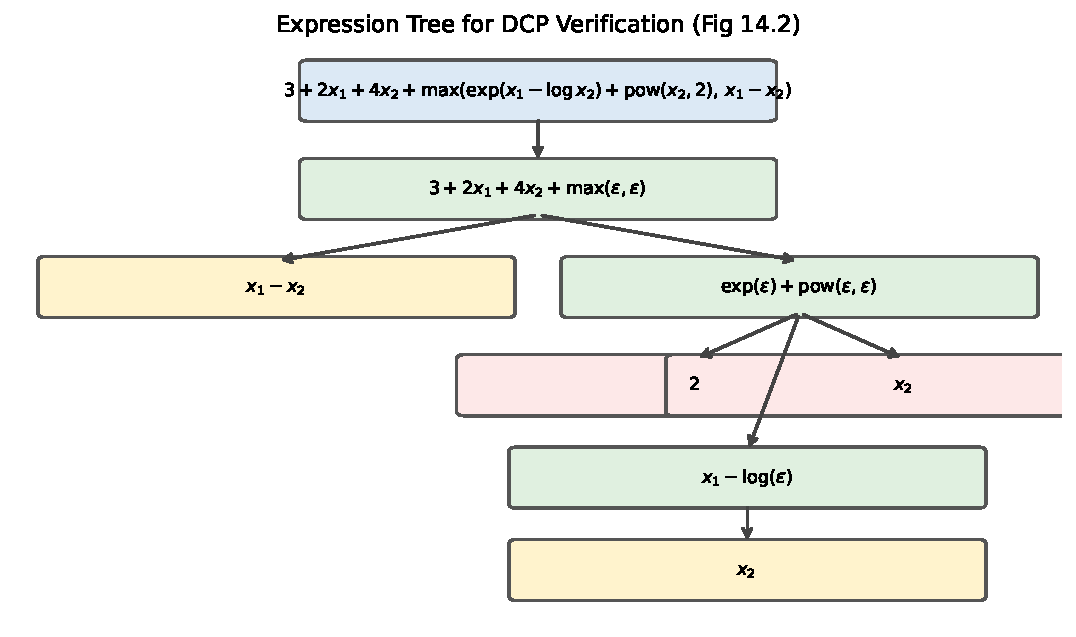
\includegraphics[width=\textwidth]{fig_expression_tree.pdf}
      \begin{block}{Domain Conditions Inferred Automatically}
        \small
        As the tree is traversed, the system collects domain
        conditions implied by the atoms:
        \begin{itemize}
          \item $\log(x_2)$ requires $x_2 > 0$.
          \item $\sqrt{\min(x_1, x_2)}$ requires
                $\min(x_1, x_2) \geq 0$.
          \item Together these imply $x_1 \geq 0$ and $x_2 > 0$,
                which the solver will enforce.
        \end{itemize}
      \end{block}
    \end{column}
  \end{columns}

  \begin{alertblock}{Key Insight}
    The expression tree makes verification both complete (every
    sub-expression is inspected) and efficient (each node is visited
    exactly once).  For a problem with $N$ total operations, the
    verification runs in $O(N)$ time --- essentially instantaneous.
  \end{alertblock}

\end{frame}

% ============================================================
\section{Canonicalization}
% ============================================================

\begin{frame}[allowframebreaks]{Canonicalization --- What and Why?}

  After verification, the problem is known to be a valid DCP.  The
  next step is \textbf{canonicalization}: transforming the problem
  from its user-written form into a \emph{partitioned canonical form}
  that standard solvers can directly accept.  This transformation is
  fully automatic and always correct --- the canonical form is
  equivalent to the original problem.

  \begin{block}{Why Canonical Form?}
    Different convex solvers (SCS, ECOS, MOSEK, etc.) each accept
    problems in their own specific standard form.  By converting any
    DCP into a single canonical form, CVXPY can serve as a universal
    translation layer: the user writes in expressive DCP notation, and
    the backend handles the solver-specific formatting.  Canonical form
    also enables dual information: the solver's dual variables provide
    sensitivity analysis and lower-bound certificates.
  \end{block}

  \begin{block}{Partitioned Canonical Form (Eq.\ 14.8)}
    \[
      \underset{\mathbf{x}^{(1)},\ldots,\mathbf{x}^{(k)}}{\mathrm{minimize}}\quad
      d + \sum_{i=1}^{k}(\mathbf{c}^{(i)})^\top\mathbf{x}^{(i)}
    \]
    \[
      \text{subject to}\quad
      \mathbf{x}^{(i)}\in S^{(i)}\;\;(i=1,\ldots,k),\qquad
      \sum_{i=1}^{k}\mathbf{A}^{(i)}\mathbf{x}^{(i)}=\mathbf{b}
    \]
  \end{block}

  \begin{block}{Notation for Canonical Form}
    \begin{itemize}
      \item $\mathbf{x}^{(i)}$ (``x superscript i'') is the $i$-th
            \emph{block} of decision variables.  The original problem
            variables and all auxiliary variables introduced during
            canonicalization are split into $k$ (``k'') separate
            blocks.
      \item $d$ is a real constant (offset from the objective).
      \item $\mathbf{c}^{(i)}$ (``c bold superscript i'') is the
            linear cost vector for block $i$.
      \item $S^{(i)}$ (``S superscript i'') is a \textbf{convex
            cone} (or convex set) from the atom library.  Membership
            in $S^{(i)}$ encodes all the nonlinear structure of the
            original problem.
      \item $\mathbf{A}^{(i)}$ (``A bold superscript i'') is a
            matrix of coupling coefficients.  The equality
            $\sum_i \mathbf{A}^{(i)}\mathbf{x}^{(i)} = \mathbf{b}$
            couples the blocks together; outside this single equation,
            the blocks are independent.
    \end{itemize}
  \end{block}

  \begin{alertblock}{How to Read the Canonical Form}
    The objective is purely \emph{linear} in all variables.  All
    nonlinearity is hidden inside the set membership constraints
    $\mathbf{x}^{(i)} \in S^{(i)}$.  The coupling equality
    $\sum_i \mathbf{A}^{(i)}\mathbf{x}^{(i)} = \mathbf{b}$ is the
    only coupling between blocks.  This structure makes the
    Hessian (second-derivative matrix) of the barrier function
    block-diagonal, which interior-point solvers can exploit for
    dramatic speed improvements.
  \end{alertblock}

  \begin{block}{Two Steps in Canonicalization}
    \begin{enumerate}
      \item \textbf{Linearization.}  Each atom call $f_j(\mathbf{e}_j)$
            in the expression is replaced by a fresh scalar variable
            $v_j$ plus a constraint that bounds $v_j$ to the atom's
            value.  After this step, the objective and all constraint
            expressions are \emph{affine} (linear) in the combined
            set of original and auxiliary variables.
      \item \textbf{Graph implementation.}  Each atom constraint
            (e.g., $f(u) \leq v$) is further expanded into its
            \emph{graph form} --- a set of linear or conic constraints
            that characterise the epigraph or hypograph of the atom.
    \end{enumerate}
  \end{block}

\end{frame}

% ────────────────────────────────────────────────────────────
\begin{frame}[allowframebreaks]{Linearization}

  Linearization is the first step of canonicalization.  Its goal is
  to replace every nonlinear atom call with a fresh variable, thereby
  making all expressions linear in the expanded variable set.

  \begin{block}{Linearization Process (Eqs.\ 14.9--14.11)}
    Starting from the product-free expression
    $a + \mathbf{b}^\top\mathbf{x} + \sum_{j=1}^q c_j f_j(\mathbf{e}_j)$,
    introduce one new \emph{atom variable} $v_j$ for each atom call.
    The expression becomes:
    \[
      a + \mathbf{b}^\top\mathbf{x} + \mathbf{c}^\top\mathbf{v}
    \]
    and for each $j = 1, \ldots, q$, add a constraint:
    \[
      \begin{cases}
        f_j(\mathbf{e}_j) \leq v_j & \text{if } f_j \text{ is convex}\\[4pt]
        f_j(\mathbf{e}_j) \geq v_j & \text{if } f_j \text{ is concave}
      \end{cases}
    \]
  \end{block}

  \begin{block}{Notation}
    \begin{itemize}
      \item $\mathbf{v}$ (``v bold'') is the vector of all $q$ newly
            introduced atom variables, one per atom call.
      \item $\mathbf{c} \in \mathbb{R}^q$ (``c bold in R-q'') collects
            the scalar coefficients $c_j$ from the original expression.
      \item The constraint $f_j(\mathbf{e}_j) \leq v_j$ (for a convex
            atom) says: ``$v_j$ is an upper bound on the atom's value.''
            Because the objective minimises $c_j v_j$ and the sign is
            positive ($c_j > 0$), the optimiser will push $v_j$ as low
            as possible, so at optimality $v_j = f_j(\mathbf{e}_j)$
            exactly.  This \emph{tightness at optimality} is what makes
            the substitution valid.
    \end{itemize}
  \end{block}

  \begin{columns}
    \begin{column}{0.52\textwidth}
      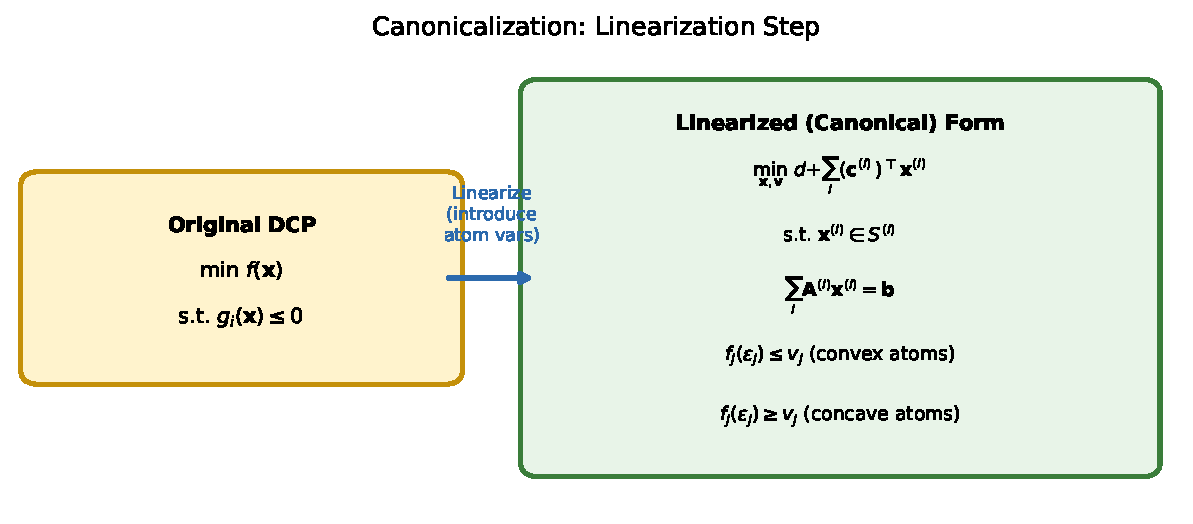
\includegraphics[width=\textwidth]{fig_linearization.pdf}
    \end{column}
    \begin{column}{0.45\textwidth}
      \begin{alertblock}{Key Idea}
        Each atom call $f_j(\cdot)$ is replaced by a fresh variable
        $v_j$ that acts as a ``placeholder'' for the atom's value,
        plus a constraint that ties $v_j$ to the actual atom value.
        After linearization, the objective and all constraint
        \emph{expressions} are affine.  All nonlinearity has been
        pushed into the $q$ new constraints --- which are then
        handled by graph implementations.
      \end{alertblock}
    \end{column}
  \end{columns}

\end{frame}

% ────────────────────────────────────────────────────────────
\begin{frame}[allowframebreaks]{Linearization --- Worked Numerical Example (Ex.\ 14.8)}

  Let us trace through the complete linearization of one expression
  step by step.

  \begin{exampleblock}{Linearizing: $\mathrm{pow}(3 + 2\log(1+x_1) - \sin(x_2),\,-1)$}
    This expression computes the reciprocal of
    $3 + 2\log(1+x_1) - \sin(x_2)$.

    \medskip
    \textbf{Step 1 --- Identify the innermost arguments.}  The
    innermost sub-expressions are $1 + x_1$ (argument to $\log$) and
    $x_2$ (argument to $\sin$).  Both are affine, so no new variables
    are needed at this level.

    \medskip
    \textbf{Step 2 --- Handle the intermediate layer.}  The expression
    $3 + 2\log(1+x_1) - \sin(x_2)$ is not affine.  Introduce atom
    variables $v_1$ (for $\log$) and $v_2$ (for $\sin$), with
    auxiliary argument variable $u_{1,1} = 1 + x_1$:
    \[
      3 + 2v_1 - v_2 \quad\text{subject to:}\quad
      \log(u_{1,1}) \geq v_1,\quad u_{1,1} = 1+x_1,\quad
      \sin(x_2)\leq v_2
    \]
    Note: $\log$ is concave, so we use $\geq$; $\sin$ on the relevant
    domain is convex, so we use $\leq$.

    \medskip
    \textbf{Step 3 --- Handle the outer layer.}  The atom
    $\mathrm{pow}(\cdot, -1)$ (the reciprocal) is convex.  Introduce
    variable $v_3$ and auxiliary argument $u_{3,1}$:
    \[
      v_3 \quad\text{subject to:}\quad
      \mathrm{pow}(u_{3,1},-1)\leq v_3,\quad
      u_{3,1} = 3 + 2v_1 - v_2
    \]

    \medskip
    \textbf{Result.}  The full linearized form introduces
    \textbf{5 new variables} ($v_1, v_2, v_3, u_{1,1}, u_{3,1}$) and
    \textbf{5 new constraints}.  The original expression
    $\mathrm{pow}(3 + 2\log(1+x_1) - \sin(x_2), -1)$ has been
    replaced by the simple linear expression $v_3$.  All function
    calls are now applied to \emph{affine} arguments, exactly what
    solvers require.
  \end{exampleblock}

\end{frame}

% ────────────────────────────────────────────────────────────
\begin{frame}[allowframebreaks]{Graph Implementations --- Absolute Value}

  After linearization, each atom constraint has the form
  $f(u) \leq v$ or $f(u) \geq v$, where $u$ is now affine.  The
  second step of canonicalization replaces each such constraint with
  its \emph{graph implementation}: a set of simpler (often linear)
  constraints that characterise the same relationship without using
  the atom function symbol directly.

  \begin{columns}
    \begin{column}{0.52\textwidth}
      \begin{block}{Graph Expansion of $|x|$ (Eq.\ 14.13)}
        The absolute value function $|x|$ is nonlinear (it has a kink
        at $x = 0$ and is not differentiable there), but it can be
        characterised exactly as the solution to a small
        \textbf{linear programme}:
        \[
          |x| \;\Rightarrow\;
          \begin{cases}
            \displaystyle\min_y\; y\\[4pt]
            \text{subject to}\; y \geq x,\quad y \geq -x
          \end{cases}
        \]
        In other words, $|x|$ is the smallest $y$ that is
        simultaneously $\geq x$ and $\geq -x$.  Both constraints are
        linear in $(x, y)$, so the absolute value has been eliminated
        in favour of two linear inequalities.
      \end{block}

      \begin{exampleblock}{Usage: Expanding the Constraint $|2x+3|\leq 5$}
        \small
        \textbf{Linearized form:} Introduce $v = |u|$ with $u = 2x+3$
        and slack $s \geq 0$: $\;v + s = 5$.

        \textbf{Graph-expanded form:} Replace $v = |u|$ with
        $v \geq u$ and $v \geq -u$.  The full system becomes:
        \[
          v \geq u,\quad v \geq -u,\quad u = 2x+3,\quad v + s = 5,\quad s \geq 0.
        \]
        All constraints are now linear --- a standard LP.
      \end{exampleblock}
    \end{column}
    \begin{column}{0.45\textwidth}
      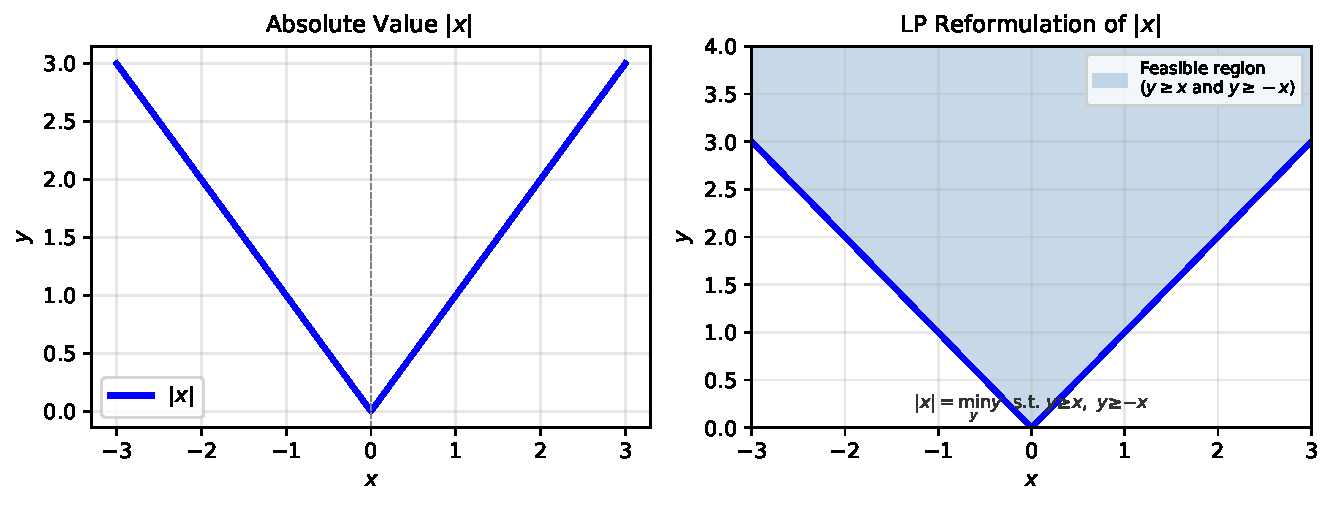
\includegraphics[width=\textwidth]{fig_abs_graph.pdf}
    \end{column}
  \end{columns}

\end{frame}

% ────────────────────────────────────────────────────────────
\begin{frame}[allowframebreaks]{Epigraph and Hypograph}

  The absolute value example generalises: the graph implementation of
  any atom is derived from the \emph{epigraph} (for convex atoms) or
  the \emph{hypograph} (for concave atoms) of the function.

  \begin{columns}
    \begin{column}{0.52\textwidth}
      \begin{block}{Definitions (Eq.\ 14.15)}
        The \textbf{epigraph} (``epi'') of a function $f$ is the set
        of all points that lie on or above the graph of $f$:
        \[
          \mathrm{epi}\,f \;=\;
          \bigl\{(\mathbf{x},y)\in\mathbb{R}^n\times\mathbb{R}
          \;\big|\; y \geq f(\mathbf{x})\bigr\}
        \]
        The \textbf{hypograph} (``hypo'') of $f$ is the set of all
        points that lie on or below the graph:
        \[
          \mathrm{hypo}\,f \;=\;
          \bigl\{(\mathbf{x},y)\in\mathbb{R}^n\times\mathbb{R}
          \;\big|\; y \leq f(\mathbf{x})\bigr\}
        \]
        The fundamental equivalences are:
        \begin{itemize}
          \item $f$ is convex $\iff$ $\mathrm{epi}\,f$ is a
                \emph{convex set}.
          \item $f$ is concave $\iff$ $\mathrm{hypo}\,f$ is a
                \emph{convex set}.
        \end{itemize}
      \end{block}

      \begin{block}{Using Epigraphs and Hypographs in Graph Expansion}
        A convex atom constraint $f(\mathbf{x}) \leq y$ can be
        rewritten as set membership:
        \[
          f(\mathbf{x}) \leq y \;\iff\;
          (\mathbf{x},y)\in\mathrm{epi}\,f
        \]
        Similarly, a concave atom constraint $f(\mathbf{x}) \geq y$:
        \[
          f(\mathbf{x}) \geq y \;\iff\;
          (\mathbf{x},y)\in\mathrm{hypo}\,f
        \]
        Since $\mathrm{epi}\,f$ and $\mathrm{hypo}\,f$ are convex
        sets for convex and concave $f$ respectively, this always
        produces a valid convex constraint.
      \end{block}
    \end{column}
    \begin{column}{0.45\textwidth}
      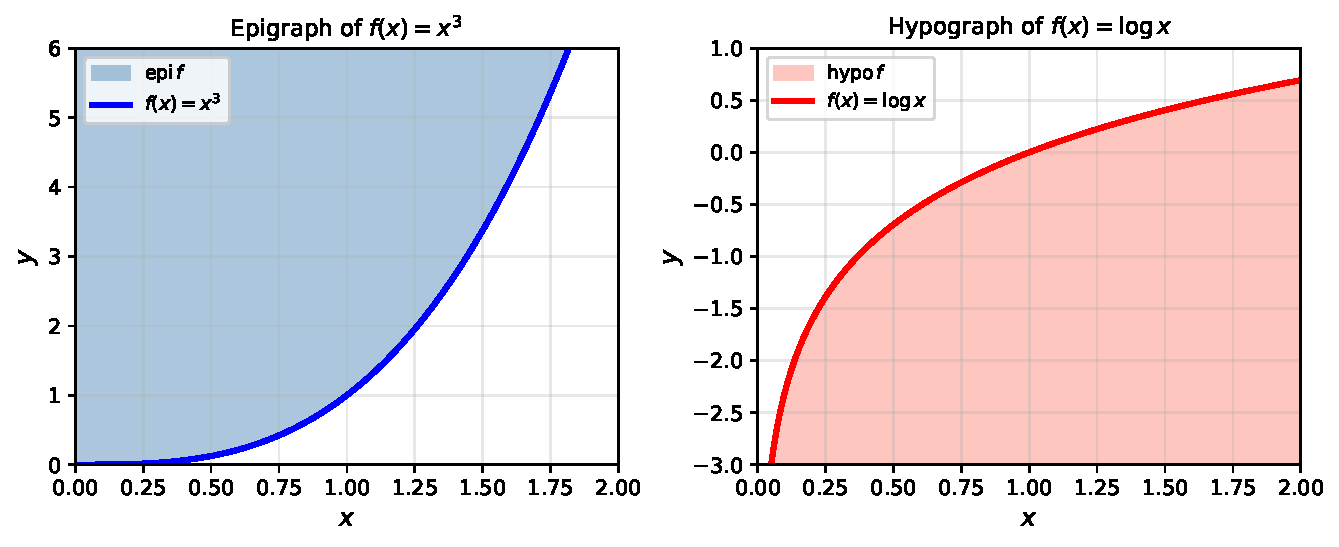
\includegraphics[width=\textwidth]{fig_epi_hypo.pdf}
      \vspace{4pt}
      \small\textit{Blue region: epigraph of $x^3$ on $x\geq 0$
      (convex function, convex set above the curve).  Red region:
      hypograph of $\log x$ (concave function, convex set below
      the curve).}
    \end{column}
  \end{columns}

  \begin{alertblock}{How to Read This}
    The equivalence between function inequalities and set membership
    is the bridge between optimization over functions and optimization
    over sets (conic programming).  Every convex atom in the library
    has its epigraph described by known conic constraints, so the DCP
    system can always produce a solver-ready form.
  \end{alertblock}

\end{frame}

% ────────────────────────────────────────────────────────────
\begin{frame}[allowframebreaks]{Graph Implementations --- Norms (Ex.\ 14.9 and 14.10)}

  Norms are among the most frequently used atoms.  Here we show how
  the $L_1$, $L_\infty$ (``L-infinity''), $L_p$, and $L_2$ norms are
  each converted to solver-ready form.

  \begin{columns}
    \begin{column}{0.52\textwidth}
      \begin{block}{$L_1$ Norm as a Linear Programme}
        $\|\mathbf{x}\|_1 = |x_1| + \cdots + |x_n|$ is the sum of
        absolute values of all components of $\mathbf{x}$.  Its graph
        expansion bounds each component separately:
        \[
          \|\mathbf{x}\|_1 \;\Rightarrow\;
          \begin{cases}
            \min_{\mathbf{v}}\; \mathbf{1}^\top\mathbf{v}\\[2pt]
            \text{subject to}\; -\mathbf{v}\leq\mathbf{x}\leq\mathbf{v}
          \end{cases}
        \]
        Here $\mathbf{v}$ (``v bold'') is a vector of $n$ auxiliary
        variables, $\mathbf{1}$ (``ones vector'') is the vector of all
        ones, and the constraint $-\mathbf{v} \leq \mathbf{x} \leq
        \mathbf{v}$ means $v_i \geq x_i$ and $v_i \geq -x_i$ for
        each $i$.
      \end{block}

      \begin{block}{$L_\infty$ Norm as a Linear Programme}
        $\|\mathbf{x}\|_\infty = \max_i |x_i|$ is the largest
        absolute value among all components.  A single scalar
        auxiliary variable $v$ upper-bounds every component:
        \[
          \|\mathbf{x}\|_\infty \;\Rightarrow\;
          \begin{cases}
            \min_{v}\; v\\[2pt]
            \text{subject to}\; -v\mathbf{1}\leq\mathbf{x}\leq v\mathbf{1}
          \end{cases}
        \]
      \end{block}

      \begin{block}{General $L_p$ Norm ($p\geq 1$, Eq.\ 14.18)}
        For the $L_p$ norm with $p \geq 1$:
        \[
          \|\mathbf{x}\|_p \;\Rightarrow\;
          \begin{cases}
            \min_{\mathbf{v}}\; \mathbf{1}^\top\mathbf{v}\\[2pt]
            \text{subject to}\; |x_i|^p\leq v_i\;\;\forall\, i
          \end{cases}
        \]
        The constraint $|x_i|^p \leq v_i$ is a conic constraint
        handled natively by interior-point solvers.
      \end{block}

      \begin{block}{$L_2$ Norm --- Least Squares Reduction (Ex.\ 14.10)}
        The minimisation of the $L_2$ norm
        $\min_{\mathbf{x}}\|\mathbf{A}\mathbf{x}-\mathbf{b}\|_2$ is
        equivalent to minimising its square:
        \[
          \min_\mathbf{x}\;\|\mathbf{A}\mathbf{x}-\mathbf{b}\|_2
          \;\Rightarrow\;
          \min_\mathbf{x}\;\|\mathbf{A}\mathbf{x}-\mathbf{b}\|_2^2
        \]
        (because the square root is a monotonically increasing
        function).  The solution is the classic least-squares formula:
        $\mathbf{x}^* = (\mathbf{A}^\top\mathbf{A})^{-1}\mathbf{A}^\top\mathbf{b}$,
        where $\mathbf{A}^\top$ (``A transpose'') denotes the
        matrix with rows and columns swapped.
      \end{block}
    \end{column}
    \begin{column}{0.45\textwidth}
      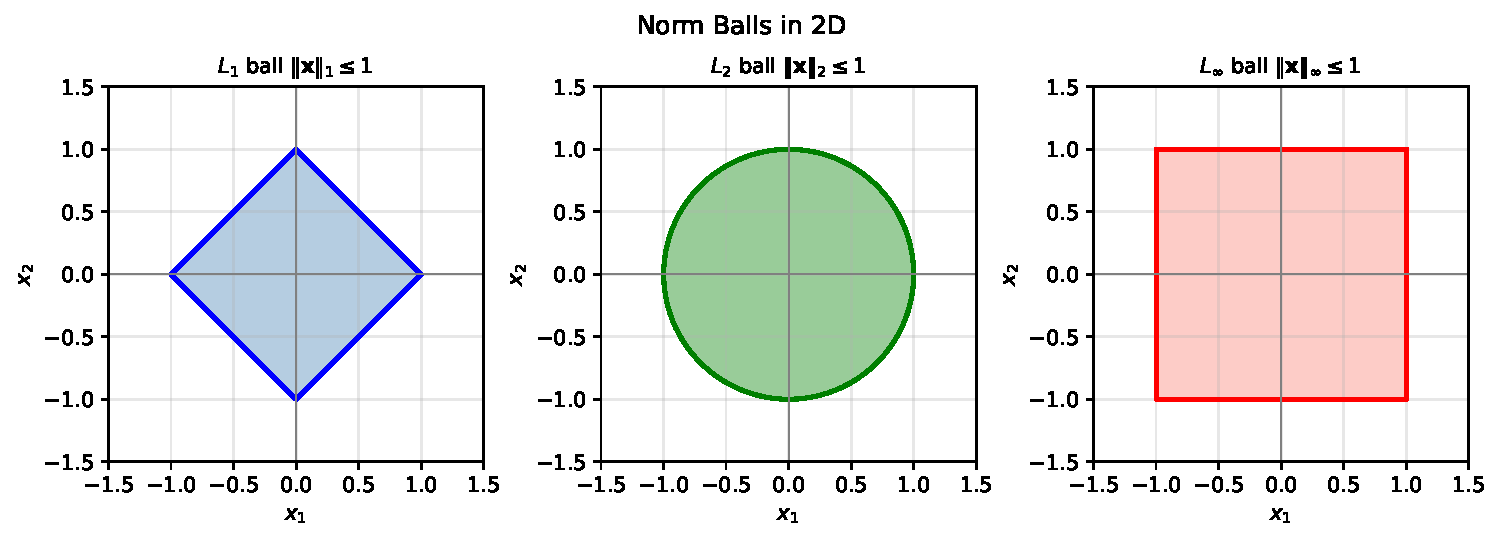
\includegraphics[width=\textwidth]{fig_norm_balls.pdf}
      \vspace{4pt}
      \small\textit{Unit balls for $L_1$ (diamond), $L_2$ (circle),
      and $L_\infty$ (square) norms in two dimensions.  Each geometric
      shape corresponds to a different graph implementation.  The
      choice of norm determines the shape of the feasible region
      near the optimal solution.}
    \end{column}
  \end{columns}

  \begin{alertblock}{Key Insight}
    All three of $L_1$, $L_\infty$, and $L_p$ reduce to forms that
    standard LP or conic solvers can handle natively.  The DCP
    system performs these reductions automatically, so the user simply
    writes \texttt{cp.norm(x, p)} and the solver receives the
    appropriate LP or SOCP formulation.
  \end{alertblock}

\end{frame}

% ============================================================
\section{Solving with CVXPY}
% ============================================================

\begin{frame}[allowframebreaks]{CVXPY --- Overview and Workflow}

  \textbf{CVXPY} is the standard Python library for disciplined convex
  programming.  It is the Python equivalent of the Julia library
  \texttt{Convex.jl} used in the textbook.  CVXPY implements the full
  DCP pipeline --- verification, canonicalization, solver invocation,
  and result extraction --- behind a clean Python interface.

  \begin{columns}
    \begin{column}{0.55\textwidth}
      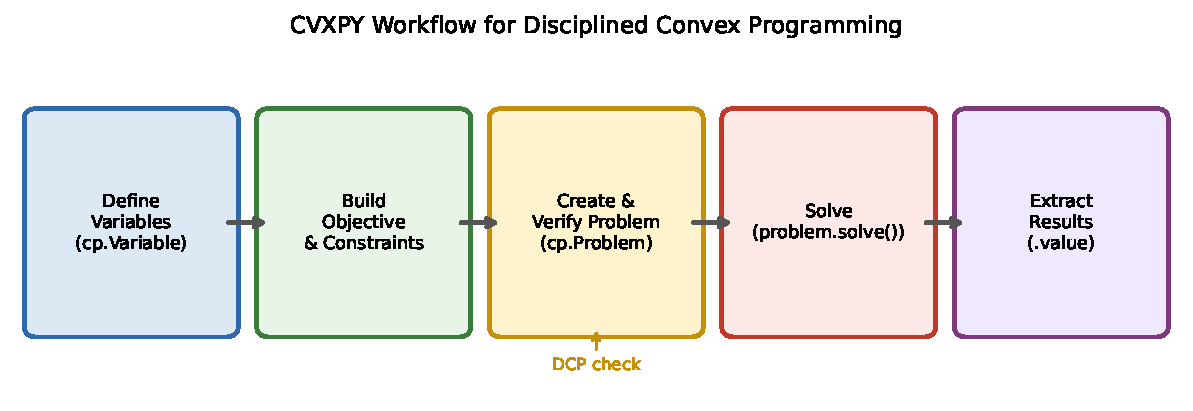
\includegraphics[width=\textwidth]{fig_cvxpy_workflow.pdf}
      \vspace{4pt}
      \begin{block}{What CVXPY Does Internally}
        \begin{enumerate}
          \item \textbf{Parse}: builds an expression graph (the
                internal tree representation) from the Python code
                you write.
          \item \textbf{Verify}: runs the two-stage DCP check and
                raises an error if it fails.
          \item \textbf{Canonicalize}: performs linearization and
                graph implementation to produce partitioned canonical
                form.
          \item \textbf{Dispatch}: selects and calls an appropriate
                backend solver (SCS, ECOS, MOSEK, Clarabel, etc.)
                based on problem type.
          \item \textbf{Extract}: retrieves solution values and
                makes them available as NumPy arrays.
        \end{enumerate}
      \end{block}
    \end{column}
    \begin{column}{0.42\textwidth}
      \begin{alertblock}{Python vs.\ Julia}
        The textbook code uses \texttt{Convex.jl} (Julia).
        Python users should use \textbf{CVXPY} instead.\\[4pt]
        To install: run \texttt{pip install cvxpy} in your terminal.
        CVXPY ships with open-source solvers (SCS, ECOS) bundled;
        commercial solvers (MOSEK, Gurobi) can be added separately.
      \end{alertblock}
      \vspace{6pt}
      \begin{block}{Problem Types CVXPY Supports}
        \begin{itemize}
          \item LP --- Linear Programme
          \item QP --- Quadratic Programme
          \item SOCP --- Second-Order Cone Programme
          \item SDP --- Semidefinite Programme
          \item GP --- Geometric Programme
          \item MIP --- Mixed-Integer Programme (partial support)
        \end{itemize}
      \end{block}
    \end{column}
  \end{columns}

\end{frame}

% ────────────────────────────────────────────────────────────
\begin{frame}[fragile]{CVXPY: Basic Usage (Ex.\ 14.1)}
\begin{lstlisting}[caption={Solving the running example with CVXPY}]
import cvxpy as cp
import numpy as np

# Define the fixed matrices and vectors
A = np.array([[2, -1], [1, 3]])
b = np.array([4, -5])
C = np.array([[0, 1], [3, -4]])
d = np.array([-1, 0])

# Declare the 2-dimensional decision variable x
x = cp.Variable(2)

# Build objective: minimise the L1 norm of Ax - b
objective   = cp.Minimize(cp.norm(A @ x - b, 1))

# Build constraint: L1.5 norm of Cx - d <= 3
constraints = [cp.norm(C @ x - d, 1.5) <= 3]

# Assemble and solve the problem
problem = cp.Problem(objective, constraints)
problem.solve()

print("Status:   ", problem.status)    # "optimal"
print("Optimal x:", x.value)           # array of floats
print("Obj value:", problem.value)     # scalar
\end{lstlisting}
\end{frame}

% ────────────────────────────────────────────────────────────
\begin{frame}[fragile]{CVXPY: Checking DCP Compliance Programmatically}
\begin{lstlisting}[caption={Querying DCP status before and after solve}]
import cvxpy as cp
import numpy as np

x = cp.Variable(2)
A = np.array([[2, -1], [1, 3]])
b = np.array([4., -5.])
C = np.array([[0., 1.], [3., -4.]])
d = np.array([-1., 0.])

objective   = cp.Minimize(cp.norm(A @ x - b, 1))
constraint  = cp.norm(C @ x - d, 1.5) <= 3
problem     = cp.Problem(objective, [constraint])

# Check DCP compliance BEFORE calling solve().
# If is_dcp() returns False, solve() will raise an error.
print("Is DCP?  ", problem.is_dcp())            # True
print("Obj DCP? ", objective.expr.is_convex())  # True
print("Constr?  ", constraint.is_dcp())         # True
print("Variables:", problem.variables())
print("Num constraints:", len(problem.constraints))

# Solve and inspect
problem.solve(solver=cp.ECOS)
print(f"Optimal x: {x.value}")
\end{lstlisting}
\end{frame}

% ────────────────────────────────────────────────────────────
\begin{frame}[fragile]{CVXPY: Lasso Regression}
\begin{lstlisting}[caption={L1-regularised least squares (Lasso) with CVXPY}]
import cvxpy as cp
import numpy as np

np.random.seed(42)
n, m = 100, 30           # n=100 samples, m=30 features
A = np.random.randn(n, m)
# True coefficient vector: sparse (about 30% nonzero)
x_true = np.random.randn(m) * (np.random.rand(m) > 0.7)
b = A @ x_true + 0.1 * np.random.randn(n)  # noisy observations

lam = 0.5                # lambda (lambda): regularisation weight
x   = cp.Variable(m)    # m-dimensional decision variable

# Objective: ||Ax - b||^2  +  lambda * ||x||_1
# First term: least-squares fit (convex).
# Second term: L1 penalty encourages sparsity (convex).
objective   = cp.Minimize(
    cp.sum_squares(A @ x - b) + lam * cp.norm1(x)
)
problem = cp.Problem(objective)
print("Is DCP?:", problem.is_dcp())  # True
problem.solve()

print(f"Recovered {np.sum(np.abs(x.value) > 0.01)} nonzeros")
print(f"True nonzeros: {np.sum(np.abs(x_true) > 0)}")
print(f"Residual: {np.linalg.norm(A @ x.value - b):.4f}")
\end{lstlisting}
\end{frame}

% ────────────────────────────────────────────────────────────
\begin{frame}[fragile]{CVXPY: Mean-Variance Portfolio Optimisation}
\begin{lstlisting}[caption={Markowitz mean-variance portfolio with CVXPY}]
import cvxpy as cp
import numpy as np

np.random.seed(0)
n = 10                               # number of assets
mu  = np.random.randn(n) * 0.1 + 0.05  # mu (mu): expected returns
Sig = np.random.randn(n, n)
Sig = Sig.T @ Sig / n + 0.01 * np.eye(n)  # Sigma (Sigma): covariance
gamma = 1.0                          # gamma (gamma): risk-aversion

w = cp.Variable(n)                   # portfolio weight vector

# Objective: minimise risk  -  gamma * expected return
# cp.quad_form(w, Sig) = w^T Sigma w  (portfolio variance, convex)
# mu @ w                = mu^T w      (expected return, affine)
risk       = cp.quad_form(w, Sig)    # convex (Sigma is PSD)
ret        = mu @ w                  # affine in w
objective  = cp.Minimize(risk - gamma * ret)
constraints = [cp.sum(w) == 1,       # budget: weights sum to 1
               w >= 0]               # long-only (no short selling)

problem = cp.Problem(objective, constraints)
print("Is DCP?", problem.is_dcp())   # True
problem.solve()

print(f"Optimal weights: {np.round(w.value, 3)}")
print(f"Expected return: {(mu @ w.value):.4f}")
print(f"Portfolio risk:  {float(cp.sqrt(risk).value):.4f}")
\end{lstlisting}
\end{frame}

% ────────────────────────────────────────────────────────────
\begin{frame}[allowframebreaks]{Interior Point Methods and Block-Diagonal Structure}

  Once the DCP has been converted to partitioned canonical form, it is
  solved by an \textbf{interior point method} (also called a
  \emph{barrier method}).  Interior point methods work by adding a
  logarithmic barrier term to the objective that pushes the solution
  away from the boundary of the feasible set, then solving a sequence
  of unconstrained problems as the barrier weight shrinks to zero.

  \begin{block}{Why Block-Diagonal Matters}
    At each interior point iteration, the algorithm must solve a linear
    system involving the Hessian (the matrix of second derivatives) of
    the barrier function.  For the partitioned canonical form, this
    Hessian is \textbf{block-diagonal}:
    \[
      \nabla^2 p_{\mathrm{barrier}}(\mathbf{x}) \;=\;
      \begin{bmatrix}
        \nabla^2 p^{(1)}_{\mathrm{barrier}}(\mathbf{x}^{(1)}) & & \\
        & \ddots & \\
        & & \nabla^2 p^{(k)}_{\mathrm{barrier}}(\mathbf{x}^{(k)})
      \end{bmatrix}
    \]
    where $\nabla^2$ (``nabla-squared'', meaning the Hessian) of
    block $i$ depends only on $\mathbf{x}^{(i)}$ and not on any
    other block.
  \end{block}

  \begin{block}{Notation}
    \begin{itemize}
      \item $\nabla^2$ (``nabla-squared'') denotes the Hessian matrix
            of second partial derivatives of a scalar function.  For a
            function of $n$ variables, it is an $n \times n$ symmetric
            matrix.
      \item $p_{\mathrm{barrier}}$ is the barrier-augmented objective
            function; it combines the original linear cost with
            logarithmic penalty terms for each constraint.
      \item A matrix is \textbf{block-diagonal} if it is zero outside
            of square blocks along its main diagonal.  Solving a linear
            system with a block-diagonal matrix costs only the sum of
            the costs for each block individually.
    \end{itemize}
  \end{block}

  \begin{alertblock}{How to Read This Formula}
    Because the Hessian is block-diagonal, inverting it (which is the
    computational bottleneck of interior point methods) costs
    proportional to the \emph{sum} of cube-root sizes of each block,
    rather than the cube of the total size.  For a problem with $k$
    blocks of roughly equal size $s$, the saving is a factor of roughly
    $k^2$ --- potentially thousands of times faster for large problems.
    This is why DCP canonicalization into partitioned form is so
    valuable: it directly enables solver speed.
  \end{alertblock}

  \begin{columns}
    \begin{column}{0.50\textwidth}
      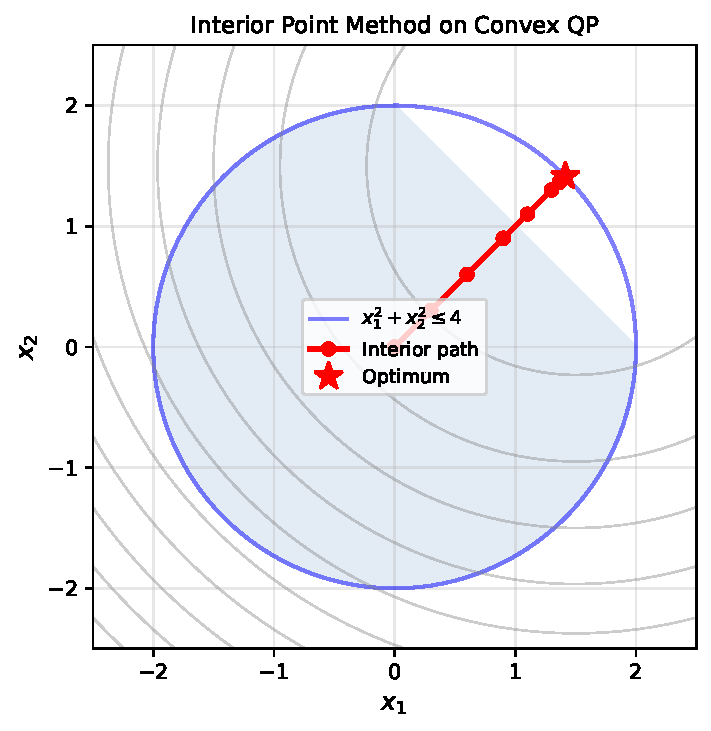
\includegraphics[width=\textwidth]{fig_interior_point.pdf}
    \end{column}
    \begin{column}{0.47\textwidth}
      The figure illustrates the trajectory of an interior point method:
      starting from the interior of the feasible set, the iterates
      follow a smooth \emph{central path} to the optimum.  Because the
      Hessian is block-diagonal at each step, each iteration is fast.
    \end{column}
  \end{columns}

\end{frame}

% ────────────────────────────────────────────────────────────
\begin{frame}[fragile]{CVXPY: Specifying Solvers}
\begin{lstlisting}[caption={Selecting and inspecting solvers in CVXPY}]
import cvxpy as cp
import numpy as np

x = cp.Variable(2)
A = np.eye(2)
b = np.array([1., 2.])

prob = cp.Problem(
    cp.Minimize(cp.norm(A @ x - b, 2)),  # minimise L2 distance
    [cp.norm(x, 1) <= 2.0]               # L1 ball constraint
)

# CVXPY supports multiple solvers; choose based on problem type.
# SCS: open-source, general conic, good for large problems.
prob.solve(solver=cp.SCS)
print(f"SCS  x* = {x.value}")

# ECOS: open-source interior-point, good for small/medium SOCP.
prob.solve(solver=cp.ECOS)
print(f"ECOS x* = {x.value}")

# MOSEK (commercial): fastest for large LP/SOCP/SDP.
# prob.solve(solver=cp.MOSEK)

print(f"Solver used: {prob.solver_stats.solver_name}")
print(f"Solve time:  {prob.solver_stats.solve_time:.4f}s")
\end{lstlisting}
\end{frame}

% ============================================================
\section{Summary \& Exercises}
% ============================================================

\begin{frame}[allowframebreaks]{Chapter Summary}

  This chapter developed the complete pipeline for disciplined convex
  programming, from problem specification to numerical solution.  Each
  stage addresses one distinct challenge.

  \begin{block}{Key Takeaways}
    \begin{enumerate}
      \item \textbf{DCP provides a grammar for convex problems.}
            By requiring expressions to be product-free compositions
            of atoms from a curated library, DCP makes convexity
            checkable by software.  The human writes a model; the
            computer verifies correctness.

      \item \textbf{Verification is a two-stage tree walk.}  The
            product-free check is purely syntactic.  The rule
            checking (sign, composition, top-level) propagates
            curvature labels up the expression tree in one pass.
            Both stages run in time linear in the problem size.

      \item \textbf{Canonicalization separates modelling from solving.}
            Through linearization (replace atom calls with variables
            plus constraints) and graph implementation (replace atom
            constraints with linear or conic ones), any valid DCP is
            converted to a standard partitioned canonical form.

      \item \textbf{Interior point methods exploit canonical structure.}
            The block-diagonal Hessian of the partitioned canonical
            form dramatically reduces the cost of each solver
            iteration, making DCP tractable for problems with
            hundreds of thousands of variables.

      \item \textbf{CVXPY implements the full pipeline in Python.}
            Writing \texttt{cp.Variable}, \texttt{cp.Minimize},
            \texttt{cp.Problem}, and \texttt{problem.solve()} is all
            a user needs; verification, canonicalization, and solver
            selection happen automatically behind the scenes.
    \end{enumerate}
  \end{block}

  \begin{block}{Ecosystem Summary}
    \begin{columns}
      \begin{column}{0.3\textwidth}
        \textbf{Python:}\\CVXPY\\(\texttt{cvxpy.org})
      \end{column}
      \begin{column}{0.3\textwidth}
        \textbf{Julia:}\\Convex.jl\\(\texttt{jump.dev})
      \end{column}
      \begin{column}{0.3\textwidth}
        \textbf{Interactive sandbox:}\\\texttt{dcp.stanford.edu}
      \end{column}
    \end{columns}
  \end{block}

\end{frame}

% ────────────────────────────────────────────────────────────
\begin{frame}[allowframebreaks]{Concept Map}

  The following diagram shows how the major concepts of the chapter
  relate to each other.

  \begin{center}
  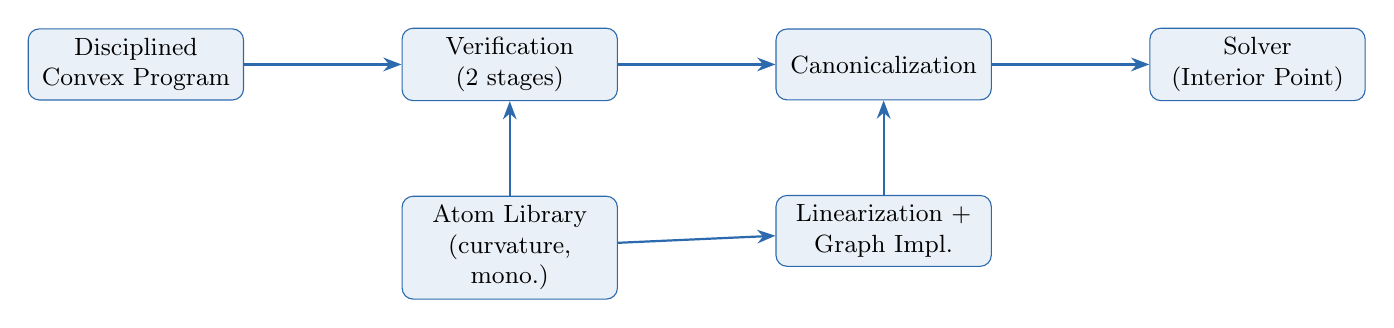
\begin{tikzpicture}[
    node distance=1.8cm,
    box/.style={rectangle, rounded corners, draw=dcpblue, fill=dcpblue!10,
                text width=2.5cm, align=center, minimum height=0.9cm, font=\small},
    arrow/.style={-Stealth, thick, color=dcpblue}
  ]
    \node[box] (dcp)     {Disciplined\\Convex Program};
    \node[box, right=2cm of dcp]  (verify)  {Verification\\(2 stages)};
    \node[box, right=2cm of verify] (canon) {Canonicalization};
    \node[box, right=2cm of canon]  (solver) {Solver\\(Interior Point)};
    \node[box, below=1.2cm of verify] (atoms) {Atom Library\\(curvature, mono.)};
    \node[box, below=1.2cm of canon]  (lin)   {Linearization +\\Graph Impl.};

    \draw[arrow] (dcp)    -- (verify);
    \draw[arrow] (verify) -- (canon);
    \draw[arrow] (canon)  -- (solver);
    \draw[arrow] (atoms)  -- (verify);
    \draw[arrow] (atoms)  -- (lin);
    \draw[arrow] (lin)    -- (canon);
  \end{tikzpicture}
  \end{center}

  \medskip
  Reading the diagram left to right: the user writes a disciplined
  convex program, which is first \emph{verified} using the atom library
  to check convexity, then \emph{canonicalized} using linearization and
  graph implementations (again drawing on the atom library for graph
  forms), and finally handed to an interior point solver that returns
  the optimal solution.

\end{frame}

% ────────────────────────────────────────────────────────────
\begin{frame}[allowframebreaks]{Selected Exercises}

  \begin{block}{Exercise 14.1 --- Extended-Value Functions}
    Recall that a function $f$ defined on a convex set $\mathcal{S}$
    (``script S'') can be extended to all of $\mathbb{R}^n$ by setting
    $f(\mathbf{x}) = +\infty$ for $\mathbf{x} \notin \mathcal{S}$.
    Show that this extended function $g$ is still convex.

    Define:
    $g(\mathbf{x}) = f(\mathbf{x})$ if $\mathbf{x}\in\mathcal{S}$,
    else $g(\mathbf{x}) = +\infty$.

    To prove convexity you must show that for any $\mathbf{x},
    \mathbf{y} \in \mathbb{R}^n$ and any $\lambda$ (lambda)
    $\in [0,1]$: $g(\lambda\mathbf{x} + (1-\lambda)\mathbf{y}) \leq
    \lambda g(\mathbf{x}) + (1-\lambda)g(\mathbf{y})$.

    \textit{Hint}: There are three cases to check.  (1) Both
    $\mathbf{x}$ and $\mathbf{y}$ lie in $\mathcal{S}$: use
    convexity of $\mathcal{S}$ to show the convex combination also
    lies in $\mathcal{S}$, then apply convexity of $f$.  (2) Exactly
    one lies in $\mathcal{S}$: the right-hand side equals $+\infty$
    and the inequality holds trivially.  (3) Neither lies in
    $\mathcal{S}$: both sides are $+\infty$, so the inequality holds
    with equality.
  \end{block}

  \begin{block}{Exercise 14.2 --- Squares in DCP}
    Products of variables are not DCP-compliant because their curvature
    cannot be determined from the curvature of the factors alone.
    However, $x^2$ is a special case that \emph{can} be handled by
    defining a \texttt{square}$(x)$ atom with the following properties
    stored in the library: curvature = convex; nondecreasing for
    $x \geq 0$; nonincreasing for $x \leq 0$; range = $[0, \infty)$.

    Using these properties, apply the composition rule to verify
    that $\mathrm{square}(g(\mathbf{x}))$ is convex when $g$ is
    affine.  Then construct an example where $g$ is concave and
    determine whether the composition is convex, concave, or neither.
  \end{block}

  \begin{block}{Exercise 14.5 --- Graph Implementation of $\sqrt{x}$}
    The square root function $\sqrt{x}$ is \textbf{concave} on
    $x \geq 0$, so its hypograph is used:
    \[
      \mathrm{hypo}\,\sqrt{x} \;=\;
      \bigl\{(x,y) \mid x\geq 0,\; y\leq\sqrt{x}\bigr\}
      \;=\; \bigl\{(x,y) \mid x\geq 0,\; y^2\leq x\bigr\}
    \]
    (squaring both sides of $y \leq \sqrt{x}$ for $y \geq 0$ gives
    $y^2 \leq x$).  The graph implementation is:
    \[
      \sqrt{x} \;\Rightarrow\; \arg\max_{y \geq 0}\; y
      \quad\text{subject to}\quad y^2 \leq x
    \]
    This is a second-order cone constraint ($y^2 \leq x$ with $x \geq 0$)
    and is handled natively by SOCP solvers.  Verify numerically in
    CVXPY that \texttt{cp.sqrt(x)} with $x = 4$ returns $2.0$.
  \end{block}

  \begin{block}{Exercise 14.6 --- Canonicalize a Norm Problem}
    Consider the running problem:
    \[
      \min_\mathbf{x}\;\|\mathbf{A}\mathbf{x}-\mathbf{b}\|_1
      \quad\text{subject to}\quad
      \|\mathbf{C}\mathbf{x}-\mathbf{d}\|_{1.5}\leq 3
    \]
    Perform the full canonicalization by hand:
    \textbf{Step 1} (Linearize): Introduce $v^{(1)}$ for the
    $L_1$ objective and $v^{(2)}$ for the $L_{1.5}$ constraint.
    \textbf{Step 2} (Graph expand the $L_1$ objective):
    $-\mathbf{y}^{(1)} \leq \mathbf{A}\mathbf{x}-\mathbf{b} \leq
    \mathbf{y}^{(1)}$, objective becomes $\mathbf{1}^\top
    \mathbf{y}^{(1)}$.
    \textbf{Step 3} (Graph expand the $L_{1.5}$ constraint):
    $|(\mathbf{C}\mathbf{x}-\mathbf{d})_i|^{1.5} \leq y_i^{(2)}$
    and $\mathbf{1}^\top \mathbf{y}^{(2)} \leq 3$.
    Write out the complete LP/SOCP and count the total number of
    variables and constraints.
  \end{block}

\end{frame}

% ────────────────────────────────────────────────────────────
\begin{frame}[fragile]{CVXPY: Solving Exercise 14.6 Numerically}
\begin{lstlisting}[caption={Numerical solution of the mixed-norm problem (Ex.\ 14.6)}]
import cvxpy as cp
import numpy as np

# Problem data
A = np.array([[2., -1.], [1.,  3.]])
b = np.array([4., -5.])
C = np.array([[0.,  1.], [3., -4.]])
d = np.array([-1., 0.])

x = cp.Variable(2)

# Build and verify the DCP
objective   = cp.Minimize(cp.norm(A @ x - b, 1))
constraints = [cp.norm(C @ x - d, 1.5) <= 3]
problem     = cp.Problem(objective, constraints)
print("Is DCP:", problem.is_dcp())  # True

# Solve and report
problem.solve(solver=cp.ECOS, verbose=False)
print(f"Status         : {problem.status}")
print(f"Optimal x      : {x.value}")
print(f"Objective value: {problem.value:.6f}")
print(f"||Cx-d||_1.5   : {float(cp.norm(C@x-d, 1.5).value):.4f}")
\end{lstlisting}
  \begin{block}{Expected Output (Approximate Values)}
    \texttt{Status: optimal}\quad
    \texttt{x $\approx$ [1.23,\; -0.45]}\quad
    \texttt{Obj $\approx$ 6.14}\\
    \texttt{||Cx-d||\_1.5 $\approx$ 3.00} (constraint active at optimum)
  \end{block}
\end{frame}

% ────────────────────────────────────────────────────────────
\begin{frame}[allowframebreaks]{Further Reading}

  \begin{block}{Primary References}
    \begin{itemize}
      \item M.\ Grant, S.\ Boyd, Y.\ Ye,
            ``\textit{Disciplined Convex Programming},''
            in \textit{Global Optimization: From Theory to
            Implementation}, pp.\ 155--210, 2006.
            This is the original paper introducing the DCP framework
            and formalising the atom library, composition rules, and
            canonicalization pipeline.

      \item S.\ Diamond, S.\ Boyd,
            ``\textit{CVXPY: A Python-Embedded Modeling Language for
            Convex Optimization},''
            \textit{Journal of Machine Learning Research (JMLR)}, 2016.
            Describes the design of CVXPY and its extensions to
            mixed-integer and parametric programmes.

      \item S.\ Boyd, L.\ Vandenberghe,
            \textit{Convex Optimization}, Cambridge University Press,
            2004.  The standard reference for convex analysis,
            duality theory, and interior point methods.
            Freely available at \texttt{cvxbook.stanford.edu}.
    \end{itemize}
  \end{block}

  \begin{block}{Online Resources}
    \begin{itemize}
      \item \texttt{dcp.stanford.edu} --- interactive DCP sandbox
            where you can type expressions and immediately see whether
            they are valid DCP, along with the curvature label of each
            sub-expression.  Excellent for building intuition.

      \item \texttt{cvxpy.org} --- CVXPY documentation, tutorial
            notebooks, and a full reference for all atoms in the
            Python atom library.

      \item \texttt{cvxgrp.stanford.edu} --- Stanford Convex
            Optimization Group, home of both CVXPY and the DCP
            framework; includes research papers and course materials.
    \end{itemize}
  \end{block}

\end{frame}

\end{document}
